\documentclass[12pt,letterpaper]{article}
\usepackage{amsmath}
\usepackage{gensymb}
\usepackage{textcomp}
\usepackage{multicol}
\usepackage{cancel}
\usepackage{enumitem}
\usepackage{graphicx}
% \renewcommand{\labelenumi}{\theparagraph.\arabic{enumi}}
\usepackage[top=1in, bottom=1in, left=0.75in, right=0.75in]{geometry}
\setlength{\parindent}{0pt}
\title{Physics Club Handout Soultions}
\begin{document}
\begin{multicols}{2}
\section{Motion}

\paragraph{Beginner problems:}
\begin{enumerate}
\item \[
\begin{aligned}
\Delta x &= \frac{v_o+v}{2}\,t\\
         &= \frac{10+20}{2}\left(10\right)\ \text{m}\\
         &= \fbox{150 m}
\end{aligned}
\]

\item \[
\begin{aligned}
\Delta r &= \sum r_i = 200\,\hat{i}\ +\\
         &  \left(135\cos{30.0\degree}\,\hat{i} + 135\sin{30.0\degree}\,\hat{j}\right) +\\
         &  \left(135\cos{-40.0\degree}\,\hat{i} + 135\sin{-40.0\degree}\,\hat{j}\right)\,\text{ft}\\
         &= \fbox{$\left(420.3\,\hat{i} - 19.28\,\hat{j}\right)$ ft}
\end{aligned}
\]

\item \[
\begin{aligned}
v_y^2&=v_{0y}+2a_y\Delta y\\
\Delta y&=\frac{v_y^2-v_{0y}^2}{2a_y}=\frac{v_0^2\sin^2 \theta}{2g}\\
v_y&=v_{0y}+a_yt\\
t&=\frac{v_y-v_{0y}}{a}=\frac{v\sin \theta}{g}\\
\Delta x &= v_{0x}t = v_0\cos \theta \frac{v_0\sin \theta}{g}
\end{aligned}
\] \[
\begin{aligned}
3 \Delta x &= \Delta y\\
3 v_0\cos \theta \frac{v_0\sin \theta}{g} &= \frac{v_0^2\sin^2 \theta}{2g}
\end{aligned}
\] \[
\begin{aligned}
\tan \theta &= 6\\
\theta &= \tan^{-1} 6 = \fbox{80.5$\degree$}
\end{aligned}
\]

\item
This question doesn't make sense.
\end{enumerate}
\paragraph{Intermediate problems:}
\begin{enumerate}
\setcounter{enumi}{4}
\item See problem 1.3.
\[
\begin{aligned}
h &= \frac{v_0^2\sin^2 \theta}{2g}\\
d &= v_0\cos \theta \frac{v_0\sin \theta}{g}\\
\frac{h}{d} &= \frac{\frac{v_0^2\sin^2 \theta}{2g}}{v_0\cos \theta \frac{v_0\sin \theta}{g}}\\
            &= \fbox{$\displaystyle \frac{\tan \theta}{2}$}
\end{aligned}
\]

\item \[
\begin{aligned}
|\vec{R}| &= \sqrt{x^2+y^2+z^2}\\
          &= \sqrt{2^2+1^2+3^2} = \fbox{3.74}
\end{aligned}
\] \[
\begin{aligned}
\cos \theta_r &= \frac{\vec{R}\,\hat{r}}{|\vec{R}|}\\
\theta_x &= \cos^{-1} \frac{\vec{R}\,\hat{i}}{|\vec{R}|} = \cos^{-1} \frac{2}{3.74} = \fbox{57.7$\degree$}\\
\theta_y &= \cos^{-1} \frac{\vec{R}\,\hat{j}}{|\vec{R}|} = \cos^{-1} \frac{1}{3.74} = \fbox{74.5$\degree$}\\
\theta_z &= \cos^{-1} \frac{\vec{R}\,\hat{k}}{|\vec{R}|} = \cos^{-1} \frac{3}{3.74} = \fbox{36.7$\degree$}
\end{aligned}
\]

\item
\vspace{-5pt}
\[
\begin{aligned}
\Delta x &= v_{0x}t\\
t &= \frac{\Delta x}{v_0\cos \theta}\\
\Delta y &= v_{0y}t + \frac{1}{2}at^2\\
\Delta y &= v_0\sin \theta \frac{\Delta x}{v_0\cos \theta} + \frac{1}{2}g\left(\frac{\Delta x}{v_0\cos \theta}\right)^2\\
\Delta y &= \tan \theta \sqrt{\left(\Delta r\right)^2 - \left(\Delta y\right)^2} +\\
         &  \frac{g\left(\left(\Delta r\right)^2 - \left(\Delta y\right)^2\right)}{2v_0^2\cos^2 \theta}\\
2.15 \times 10^3 &= \tan \theta\\
         &  \sqrt{\left(4 \times 10^3\right)^2 - \left(2.15 \times 10^3\right)^2} +\\
         &  \frac{9.81 \left(\left(4 \times 10^3\right)^2 - \left(2.15 \times 10^3\right)^2\right)}{2\cdot 280^2\cos^2 \theta}\\
\theta &= \fbox{21.5\degree}
\end{aligned}
\]
\end{enumerate}
\paragraph{Advanced problems:}
\begin{enumerate}
\setcounter{enumi}{7}
\item
$$\left(v\sin \theta\right)^2-\left(v\sin \theta\right)_0^2=2ah$$
$$\left(v\sin \theta\right)^2\propto h$$
$$v\sin\theta\propto\sqrt{h}$$
$$v_0 \cos \theta = \sqrt{\frac{6}{7}}\sqrt{\left(\frac{v_o\sin\theta}{\sqrt{2}}\right)^2+\left(v_0\cos\theta\right)^2}$$
$$cos^2 \theta = \frac{6}{7}\left(\frac{\sin^2 \theta}{2}+cos^2 \theta\right)$$
$$7cos^2 \theta = 3\sin^2 \theta + 6\cos^2 \theta$$
$$\tan \theta = \frac{1}{\sqrt{3}}$$
$$\theta = \tan^{-1} \frac{1}{\sqrt{3}} = \fbox{30$\degree$}$$


\item See problem 1.8.
$$v\sin\theta\propto\sqrt{h}$$
$$v_0 \cos \theta = m\sqrt{\left(\sqrt{n}v_o\sin\theta\right)^2+\left(v_0\cos\theta\right)^2}$$
$$cos^2 \theta = m^2\left(n\sin^2 \theta+cos^2 \theta\right)$$
$$\left(1-m^2\right)cos^2 \theta = nm^2\sin^2 \theta$$
$$\theta = \fbox{$\displaystyle \tan^{-1} \frac{1}{m}\sqrt{\frac{1-m^2}{n}}$}$$

\item \[
\begin{aligned}
x &= \left(v_0\cos \theta\right)t = d\cos \psi\\
y &= \left(v_0\sin \theta\right)t-\frac{1}{2}gt^2 = -d\sin \psi
\end{aligned}
\]
$$\left(v_0\sin \theta\right)\frac{d\cos \psi}{v_0\cos \theta}-\frac{1}{2}g\left(\frac{d\cos \psi}{v_0\cos \theta}\right)^2 = -d\sin \psi$$
$$\tan \theta \cos \psi-\frac{gd\cos^2 \psi}{2v_0^2\cos^2 \theta} = -\sin \psi$$
$$d = \frac{v_0^2}{g}\left(\sin 2\theta \sec \psi+2\cos^2 \theta\sec \psi \tan \psi\right)$$
Taking the derivative with respect to $\theta$:
$$\frac{dd}{d\theta} = \frac{2 v_0^2 \sec^2 \psi \cos\left(2 \theta+\psi\right)}{g}$$
Next, we equate this to 0 to find where $d$ is maximized. As an exercise, confirm that $d$ is at a maximum and not a minimum by computing $d^2d$\slash $d\theta^2$.
$$\frac{2 v_0^2 \sec^2 \psi \cos\left(2 \theta+\psi\right)}{g} = 0$$
$$2 \theta+\psi = \pi$$
$$\fbox{$\displaystyle \theta = \frac{\pi-\psi}{2}$}$$


\item\[
\begin{aligned}
R &= \frac{1}{2}gt^2\\
t &= \sqrt{\frac{2R}{g}}\\
\Delta x &= vt = \fbox{$\displaystyle v \sqrt{\frac{2R}{g}}$}\\
\Delta x &> R\\
v \sqrt{\frac{2R}{g}} &> R\\
v &> \sqrt{\frac{gR}{2}}
\end{aligned}
\]
\end{enumerate}

\section{Newton's Laws}

\paragraph{Beginner problems:}
\begin{enumerate}
\item
$$\sum \vec{F} = m\vec{a} = 0$$
$$\vec{F}_{air} = -\vec{v}^{\,2}*0.3141\frac{\text{kg}}{\text{m}} = mg$$
\[
\begin{aligned}
\vec{v} &= \sqrt{\frac{50\cdot 9.81}{0.3141}}\ \text{m\slash s}\\
        &= \fbox{39.5 m\slash s}
\end{aligned}
\]

\item
$$a_c = \frac{v^2}{r} = \frac{4^2}{12}\ \frac{\text{m}}{\text{s}^2} = \fbox{1.33 m\slash s$^2$}$$
\[
\begin{aligned}
a &= a_c + a_\perp = \left(1.33\,\hat{r} + 1.2\,\hat{t}\right)\,\text{m\slash s}^2\\
  &= \fbox{1.67 m\slash s$^2$ at $\theta = 48\degree$}
\end{aligned}
\]

\item \[
\begin{aligned}
F     &= ma\\
2T-mg &= m\frac{v^2}{R}
\end{aligned}
\] \[
\begin{aligned}
v &= \sqrt{R\left(\frac{2T}{m}-g\right)}\\
  &= \sqrt{3.00\left(\frac{2\cdot 350}{40.0}-9.81\right)}\ \text{m\slash s}\\
  &= \fbox{4.80 m\slash s}
\end{aligned}
\] \[
\begin{aligned}
            E_i &= E_f + W_{nc}\\
\frac{1}{2}mv^2 &= mgh
\end{aligned}
\]
$$h = \frac{v^2}{2g} = \frac{4.80^2}{2\cdot 9.81}\ \text{m} = \fbox{1.18 m}$$
\end{enumerate}

\paragraph{Intermediate problems:}
\begin{enumerate}
\setcounter{enumi}{3}
\item This question doesn't make sense.

\item
An amusement park ride is set up as a giant swing that starts at an angle of 80\degree\ to the vertical, and allows the swing to fall freely. For legal reasons, the maximum g-force a rider can experience is 5 g's (where 1 g = 9.81 m\slash s$^2$). Assuming no air resistance, what is the largest they can make the swing and still avoid litigation?

\item
A plumb bob (a weight hanging from a string) usually does not hang perfectly vertically (i.e. along a line directed towards the center of the earth). By how much does a plumb bob deviate from vertical here in Palo Alto (latitude of 37.4\degree\,N), assuming the earth is spherical and has radius 6380 km?
\end{enumerate}

\paragraph{Advanced problems:}
\begin{enumerate}
\setcounter{enumi}{6}
\item
An object moving througha a fluid experiences a force $\vec{F}_{drag} = -(ar\vec{v} + br^2\vec{v}^2)$ exerted on a sphere of radius $r$ moving through a fluid at speed $v$, where $a$ and $b$ are constants based on the shape of the object and the surrounding atmosphere. For spherical objects in air at sea level, $a = 3.10 \times 10^{-4}\,\text{Pa}\cdot \text{s}$ and $b = 0.870$ g\slash L.
Find the velocity of a water droplet of 100 \textmu m freefalling at time $t$, where $t$ is the time elapsed since it was released from rest.

% $$m\vec{g} - \vec{F}_{drag} = m\vec{a}$$
% $$v = \int a\,dt = \int \frac{F}{m}\,dt = \int_0^t \frac{m\vec{g} - (ar\vec{v} + br^2\vec{v}^2)}{m} \,dt = gt$$

\item \[
\begin{aligned}
\sum F = ma\\
F_n + F\sin \theta - mg = 0\\
F\cos \theta - f = 0\\
F\cos \theta - \mu_s\left(mg - F\sin \theta\right) = 0\\
F = \frac{\mu_s mg}{\cos \theta + \mu_s \sin \theta}
\end{aligned}
\]
In order to minimize $F$, we maximize the denominator on the right hand side by taking a derivative:
\[
\begin{aligned}
& -\sin \theta + \mu_s \cos \theta = 0\\
\theta &= \tan^{-1} \mu_s = \tan^{-1} 0.4 = \fbox{21.8$\degree$}\\
F &= \frac{\mu_s mg}{\cos \theta + \mu_s \sin \theta}\\
  &= \frac{0.4\cdot 1\cdot 9.81}{\cos 21.8\degree + 0.4 \sin 21.8\degree}\ \text{N}\\
  &= \fbox{3.64 N}
\end{aligned}
\]

\item \[
\begin{aligned}
\vec{F} &= (8.00\,\hat{i}-4.00\,t\,\hat{j})\ \text{N}\\
\vec{F} &= m\vec{a}\\
\vec{a} &= (4.00\,\hat{i}-2.00\,t\,\hat{j})\ \text{m\slash s}^2
\end{aligned}
\] \[
\begin{aligned}
\vec{v} = \int \vec{a}\,dt &= \int (4.00\,\hat{i}-2.00\,t\,\hat{j})\ \text{m\slash s}^2\,dt\\
                           &= (4.00\,t\,\hat{i}-1.00\,t^2\,\hat{j}+\cancel{C})\ \text{m\slash s}\\
|\vec{v}| = 15\ \text{m\slash s} &= \sqrt{\left(4.00\,t\right)^2+\left(-1.00\,t^2\right)^2}\\
t &= \fbox{3 s}\\
\vec{x} = \int \vec{v}\,dt &= \int (4.00\,t\,\hat{i}-1.00\,t^2\,\hat{j})\ \text{m\slash s}\, dt\\
                            &= (2.00\,t^2\,\hat{i}-0.33\,t^3\,\hat{j})\ \text{m}\\
\vec{x}\,(3\ \text{s}) &= (2.00\cdot 3^2\,\hat{i}-0.33\cdot 3^3\,\hat{j})\ \text{m}\\
&= \fbox{$18.0\,\hat{i}-9.00\,\hat{j}$ m}
\end{aligned}
\]
\end{enumerate}

\section{Energy}

\paragraph{Beginner problems:}
\begin{enumerate}
\item
\begin{enumerate}[label=(\alph*)]
\item
$\displaystyle W = F \Delta x \cos \theta$
$$W = 16.0 \cdot 2.20 \cos -25.0\degree\ \text{J} = \fbox{31.9 J}$$

\item The normal force is perpendicular to the direction of movement so the dot product $W = F \cdot \Delta x$ is \fbox{0}.

\item Similarly, the gravitational force is perpendicular to the direction of movement so the work done is \fbox{0}.

\item \(
\begin{aligned}
\displaystyle W_{\text{net}} &= W_F + W_{F_n} + W_g\\
               &= 31.9 + 0 + 0\ \text{J} = \fbox{31.9 J}
\end{aligned}
\)
\end{enumerate}

\item \[
\begin{aligned}
W &= \int F\,dx\\
  &= \int_{x = 0}^{0.600\ \text{m}} \left(5000+10000x-25000x^2\right)\,dx\\
  &= 5000x+5000x^2-8333x^3\Biggr|_{x = 0}^{0.600\ \text{m}}\ \text{J}\\
  &= \fbox{3000 J}
\end{aligned}
\]
$$\sum W = \Delta K = \frac{1}{2}mv^2$$
$$v =\sqrt{\frac{2W}{m}}=\sqrt{\frac{2\cdot 3000}{100 \times 10^{-3}}}\ \text{J} = \fbox{60000 J}$$

\item
$$E_i=E_f$$
$$\frac{1}{2}mv_0^2 + mgh = \frac{1}{2}mv^2$$
\[
\begin{aligned}
v &= \sqrt{v_0^2 + 2gh}\\
  &= \sqrt{42^2 + 2\cdot 9.81\cdot 100}\ \text{m\slash s} = \fbox{3726 m\slash s}
\end{aligned}
\]
\end{enumerate}
\paragraph{Intermediate problems:}
\begin{enumerate}
\setcounter{enumi}{3}
\item
$$W = F\,dx = -U$$
\[
\begin{aligned}
F = -U \frac{d}{dx} &= -\left(-x^3+2x^2+3x\right) \frac{d}{dx}\\
                    &= \fbox{$\displaystyle 3x^2-4x-3$}
\end{aligned}
\]
To find the stable and unstable equilibria, take the derivative of $U$ with respect to $x$:
$$U \frac{d}{dx} = -3x^2+4x+3 = 0$$
$$x = \frac{2 \pm \sqrt{13}}{3}$$
To determine whether each root is at a stable, unstable, or neutral equilibrium, we take the second derivative of $u$ with respect to $x$, $d^2U$\slash $dx^2$:
$$U \frac{d^2}{dx^2} = -6x+4$$
At $x = \frac{1}{3}\left(2 + \sqrt{13}\right)$, $d^2U$\slash $dx^2 = -\sqrt{13}$. At $x = \frac{1}{3}\left(2 - \sqrt{13}\right)$, $d^2U$\slash $dx^2 = \sqrt{13}$.
$x = \frac{1}{3}\left(2 + \sqrt{13}\right)$ is at a local maximum so it is at an unstable equilibrium.\\
$x = \frac{1}{3}\left(2 - \sqrt{13}\right)$ is at a local minimum so it is at a stable equilibrium. 

\item
$$\sum F = ma_c$$
$$F_{n,\text{bot}}-mg=m\frac{v^2}{r}$$
$$F_{n,\text{bot}} = \fbox{$\displaystyle m\left(\frac{v^2}{r}+g\right)$}$$
$$E_i=E_f$$
$$\frac{1}{2}mv^2=\frac{1}{2}mv_{\text{top}}^2+mg\left(2r\right)$$
$$v_{\text{top}}^2=v^2-4gr$$
$$\sum F = ma_c$$
$$F_{n,\text{top}}+mg=m\frac{v_{\text{top}}^2}{r}$$
\[
\begin{aligned}
F_{n,\text{top}} &= m\left(\frac{v^2-4gr}{r}-g\right)\\
&= \fbox{$\displaystyle m\left(\frac{v^2}{r}-5g\right)$}
\end{aligned}
\]

\item
A block of mass $M$ rests on a table. It is fastened to the lower end of a light, vertical spring with spring constant $k$. The upper end of the spring is fastened to a block of mass $m$. The spring is then compressed a distance $d$ (relative to its unstretched state) by pushing down on the upper block. In this configuration, the upper block is released from rest. The spring lifts the lower block off the table. In terms of $m$, what is the greatest possible value for $M$?
\end{enumerate}
\paragraph{Advanced problems:}
\begin{enumerate}
\setcounter{enumi}{6}
\item The problem requires knowledge of techniques in multivaribale calculus. Compute when $z' = 0$ to find equilibria, and compute the sign of $z''$ to find the type of equilibrium. You should get infinite solutions since $\cos$ is periodic. Some solutions include $(-3.78416, -25.736)$ and $(1.77245, 1.77245)$.\\
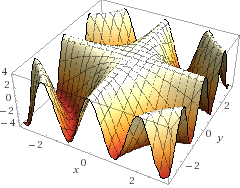
\includegraphics[width=2.5in]{3-7.png}
\item
A ball of mass 300 g is connected by a strong string of length 80.0 cm to a pivot and held in place with the string vertical. A sudden gust of wind exerts constant force $F$ to the right on the ball. The ball is released from rest. The wind makes it swing up to attain maximum height $H$ above its starting point before it swings down again. Find $H$ as a function of $F$.

\item
Two stars of mass $M$ are separated by a distance $d$. One star is moving at a velocity $v$ relative to the other star, in a direction perpendicular to the line connecting the two stars. As time approaches infinity, how will the stars behave? (Will they enter a stable orbit with one another, will they collide, will they fly apart and never meet again?)
\end{enumerate}

\section{Momentum \& Impulse}

\paragraph{Beginner problems:}
\begin{enumerate}
\item \[
\begin{aligned}
p_i&=p_f\\
\left(m_{\text{man}}+m_{\text{box}}\right)v_i&=m_{\text{man}}v+m_{\text{box}}v_{\text{box}}\\
\end{aligned}
\] \[
\begin{aligned}
v&=\frac{\left(m_{\text{man}}+m_{\text{box}}\right)v_i-m_{\text{box}}v_{\text{box}}}{m_{\text{man}}}\\
 &=\frac{\left(60+20\right)7-20\cdot 5}{60}\ \text{m\slash s}\\
 &=\fbox{7.67 m\slash s}
\end{aligned}
\]

\item \[
m = m \cdot \frac{\left(mv\right)^2}{m^2v^2} = \frac{p^2}{2K} = \frac{40^2}{2\cdot 100}\ \text{kg} = \fbox{8 kg}
\]

\item Assume your mass $m=50$ kg.
\[
\begin{aligned}
E_i &= E_f\\
\frac{1}{2}mv^2 &= mgh\\
v &= \sqrt{2gh}\\
p_i &= p_f\\
m\sqrt{2gh} &= M_EV_E
\end{aligned}
\] \[
\begin{aligned}
V_E &= \frac{m}{M_E}\sqrt{2gh}\\
&= \frac{50\sqrt{2\cdot 9.81\cdot 0.75}}{5.97\times 10^{24}}\ \text{m\slash s} = \fbox{3.22 m\slash s}
\end{aligned}
\]
\end{enumerate}
\paragraph{Intermediate problems:}
\begin{enumerate}
\setcounter{enumi}{3}
\item
$$J = \Delta p = mv = \int F\,dt$$
\[
\begin{aligned}v &= \frac{1}{m} \int F\,dt = \frac{1}{50} \int_0^4 10\, t^2\, dt\\
    &= \frac{1}{50} \frac{10}{3}\, t^3\Biggr|_0^4\ \text{m\slash s} = \fbox{4.27 m\slash s}
\end{aligned}
\]

\item \[
\begin{aligned}
\sum F &= ma\\
F_n - mg &= 0
\end{aligned}
\] \[
\begin{aligned}
E_i &= E_f+W_{nc}\\
\frac{1}{2}mv_0^2 &= \frac{1}{2}mv_1^2+\mu_k mgd_1
\end{aligned}
\]
$$v_1 = \sqrt{v_0^2-2\mu_k gd_1}$$
\[
\begin{aligned}
p_i &= p_f\\
mv_1 &= Mv_2
\end{aligned}
\]
$$v_2 = \frac{m}{M}v_1 = \frac{m}{M}\sqrt{v_0^2-2\mu_k gd_1}$$
\[
\begin{aligned}
E_i &= E_f+W_{nc}\\
\frac{1}{2}mv_2^2 &= \mu_k mgd_2
\end{aligned}
\] \[
\begin{aligned}
d_2 &= \frac{v_2^2}{2\mu_k g} = \frac{\left(\frac{m}{M}\sqrt{v_0^2-2\mu_k gd_1}\right)^2}{2\mu_k g}\\
&= \left(\frac{m}{M}\right)^2\left(\frac{v_0^2}{2\mu_k g} - d_1\right)\\
&= \left(\frac{5.0}{15.0}\right)^2\left(\frac{8.0^2}{2\cdot 0.35\cdot 9.81} - 2.0\right)\ \text{m}\\
&= \fbox{2.44 m}
\end{aligned}
\]

\item \[
\begin{aligned}
p_i &= p_f\\
mv_{1i} &= mv_{1f} + mv_{2f}\\
v_{1i} &= v_{1f} + v_{2f}\\
E_i &= E_f\\
\frac{1}{2}mv_{1i}^2 &= \frac{1}{2}mv_{1f}^2 + \frac{1}{2}mv_{2f}^2\\
v_{1i}^2 &= v_{1f}^2 + v_{2f}^2\\
\left(v_{1f} + v_{2f}\right)^2 &= v_{1f}^2 + v_{2f}^2\\
v_{1f}^2 + v_{1f} \cdot v_{2f} + v_{2f}^2 &= v_{1f}^2 + v_{2f}^2\\
v_{1f} \cdot v_{2f} &= 0
\end{aligned}
\]
$$v_{1f} \perp v_{2f}$$
\end{enumerate}
\paragraph{Advanced problems:}
\begin{enumerate}
\setcounter{enumi}{6}
\item
$$F = \frac{dp}{dt} = \frac{d\left(mv\right)}{dt} = v\,\frac{dm}{dt} + m\,\frac{dv}{dt}$$
$$dm = \frac{M}{L}\,dx$$
$$F = v\,\frac{dm}{dt}=v\left(\frac{M}{L}\right)\frac{dx}{dt} = \left(\frac{M}{L}\right)v^2$$
$$F = \frac{2Mgx}{L}$$
$$F_g = \frac{Mgx}{L}$$
$$x = \frac{1}{2}gt^2$$
$$F_{\text{net}} = F + F_g = \frac{3Mgx}{L} = \frac{3Mgx}{L} = \fbox{$\displaystyle \frac{3Mg^2t^2}{2L}$}$$


\item
Two objects of mass $m_1$ and $m_2$ are traveling at velocities $\vec{v}_1$ and $\vec{v}_2$, respectively. They undergo a completely elastic collision. Find, in terms of these quantities, the final velocities of each mass.

\item
A tennis ball of mass $m_1$ is on top of a basketball of mass $m_2$ and radius $r$. If they are dropped from a height $h$, to what height does the tennis ball bounce, assuming all collisions are elastic?

Now consider a stack of $N$ balls, where the bottom ball has mass $m$, radius $r$, and each subsequent ball has mass 1/27 that of the previous ball, and radius 1/3 that of the previous ball. Assuming all collisions are elastic and without air resistance (which is completely absurd), and the stack of balls is dropped from height $h$, what is the highest ball's velocity?

\end{enumerate}
\end{multicols}
\end{document}